\documentclass{standalone}
\usepackage{tikz}

\begin{document}

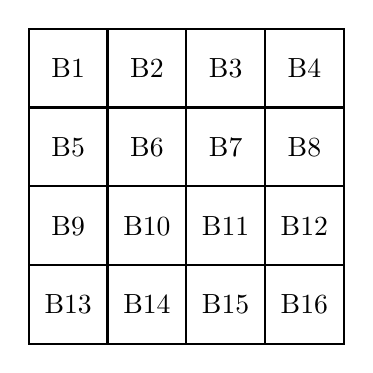
\begin{tikzpicture}

    % Draw the large square
    \draw[thick] (0, 0) rectangle (4, 4);
    
    % Draw the vertical and horizontal lines to divide the square into 16 smaller squares
    \draw[thick] (1, 0) -- (1, 4);
    \draw[thick] (2, 0) -- (2, 4);
    \draw[thick] (3, 0) -- (3, 4);
    \draw[thick] (0, 1) -- (4, 1);
    \draw[thick] (0, 2) -- (4, 2);
    \draw[thick] (0, 3) -- (4, 3);

    % Add labels inside each small square
    \foreach \i in {0,1,2,3} {
        \foreach \j in {0,1,2,3} {
            \node at (\i + 0.5, 3 - \j + 0.5) {B\the\numexpr4*\j + \i + 1\relax};
        }
    }

\end{tikzpicture}

\end{document}


